\documentclass[12pt,a4paper,titlepage]{article}
\usepackage[utf8]{inputenc}
\usepackage[T1]{fontenc}
\usepackage[top=3cm, bottom=3cm, left=2cm, right=2cm]{geometry}
\usepackage{textcomp}
\usepackage{amsmath}
\usepackage{amsfonts}
\usepackage{amssymb}
\usepackage{amsthm}
\usepackage{titlesec}
\usepackage{fancyhdr}
\usepackage{lastpage}
\usepackage{fix-cm}
\usepackage{graphicx}
\usepackage{hyperref}
\usepackage{xcolor}
\usepackage{mdwlist}
\usepackage{listings}
\usepackage{float}
\usepackage{wrapfig}
\usepackage{datetime}
\usepackage[perpage,para,bottom,marginal]{footmisc}
\usepackage{listings}
\usepackage{caption}
\usepackage{enumitem}
\usepackage{multicol}
\usepackage[cmtip,all]{xy}
\newdateformat{dmny}{\monthname[\THEMONTH] \THEYEAR}
\newdateformat{dyo}{\THEYEAR}
\setlength{\headheight}{30pt}
\pagestyle{fancy}

\author{Nicolas Hafner}
\lhead{Nicolas Hafner}
\title{Analysis II}
\chead{Analysis II}
\rhead{Zürich, \dmny\today}
\cfoot{\thepage\ / \pageref{LastPage}}
\lfoot{\copyright \dyo\today TymoonNET/NexT}
\date{\d_mny\today}

\newcommand{\longsquiggly}{\xymatrix{{}\ar@{~>}[r]&{}}}
\renewcommand{\Re}{\operatorname{Re}}
\renewcommand{\Im}{\operatorname{Im}}
\renewcommand{\arg}{\operatorname{arg}}
\renewcommand{\d}{\partial}
\newcommand{\arsinh}{\operatorname{arsinh}}
\newcommand{\arcosh}{\operatorname{arcosh}}
\newcommand{\artanh}{\operatorname{artanh}}
\newcommand{\setC}{\mathbb{C}}
\newcommand{\setR}{\mathbb{R}}
\newcommand{\setZ}{\mathbb{Z}}
\newcommand{\setN}{\mathbb{Z}^{\geq0}}
\newcommand{\Graph}{\operatorname{Graph}}

\begin{document}	
\begin{center}{\bfseries\Huge Analysis II - 2014.03.27}\end{center}
Seien $g_1..g_r:U\to\setR$ diffbar, $U\subset\setR^n$ offen, $B:=\{x\in U\mid g_1(x)=...=g_r(x)=0\}$. \\
\\
\textit{Beispiel}: $g_i$ linear $\Rightarrow B$ linearer Teilraum. \\
$\forall\xi\in B \Rightarrow$ für $x\to\xi$ mit $x\in B: \quad \underbrace{g_i(x)}_{=0}= \underbrace{g_i(\xi)}_{=0}+\langle\nabla g_i(\xi),\;x-\xi\rangle+o(|x-\xi|)$ \\
$\Rightarrow \langle\nabla g_i(\xi),\;\frac{x-\xi}{|x-\xi|}\rangle\to 0$ \\
\\
\textit{Definition}: Ein Punkt $\xi\in B$, für den $\nabla g_1(\xi)..\nabla g_r(\xi)$ linear unabhängig sind, heisst \emph{regulärer Punkt von $B$}. \\
\\
\textit{Definition/Satz}: Der Tangentialraum von $B$ in einem regulären Punkt $\xi\in B$ ist der $(n-r)$ dimensionale affin-lineare Unterraum $\{x\in\setR^n\mid\forall i=1..r:\langle\nabla g_i(\xi),x-\xi\rangle = 0\}$. \\
\\
\textit{Beispiel}: $g(x,y)=x^2-y^2-x^4 \quad \nabla g=(2x-4x^3,-2y)$ \\
\begin{figure}[h!]
  \centering
  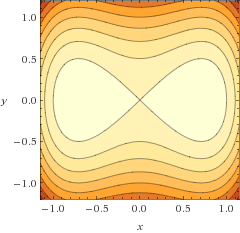
\includegraphics[keepaspectratio=true,scale=0.75]{WolframAlpha--x_2_y_2_x_4__Contour_plot__2014_03_27_0433.png}
  \caption{Singularität in $(0,0)$}
\end{figure} \\
Tangentialraum = Tangente in $(\xi,\eta):(\xi-4\xi^3)(x-\xi)-2\eta(y-\eta)=0$ \\
\\
\textit{Beispiel}: $S^2:=\{(x,y,z)\in\setR^3\mid \underbrace{x^2+y^2+z^2-1}_{g(x,y,z)}=0\} $ \\
$\Rightarrow \nabla g=(2x,2y,2z) \Rightarrow S^2$ überall regulär. \\
Tangentialebene in $(\xi,\eta,\zeta)\in S^2: 2\xi(x-\xi)+2\eta(y-\eta)+2\zeta(z-\zeta)=0$ \\
\\
\newpage
\textit{Beispiel}: $F$ gegeben durch $g(x,y,z):=x^2+y^2-z^2=0 \quad \nabla g=(2x,2y,-2z)$
\begin{figure}[h!]
  \centering
  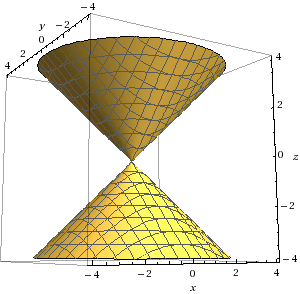
\includegraphics[keepaspectratio=true,scale=0.6]{WolframAlpha--plot_x_2_y_2_z_2_0__Surface_plot__2014_03_27_0446.png}
  \caption{Singularität in $(0,0,0)$}
\end{figure}\\
\\
\textit{Beispiel}: $\begin{array}{ll}g_1(x,y,z):=x^2+y^2+z^2-1 & \Rightarrow \nabla g_1=(2x,2y,2z)\\
  g_2(x,y,z):=x^3+y^3+z^3 & \Rightarrow \nabla g_2(x,y,z)=(3x^2,3y^2,3z^2)
\end{array}$ \\
Regulärer Punkt $\iff g_1=g_2=0$ und $\nabla g_1,\nabla g_2$ lin. unabhängig. Wenn $\nabla g_1,\nabla g_2$ lin. abhängig, so sind $x=y=z \Rightarrow 3x^2=1 \Rightarrow x=\frac{1}{\sqrt{3}} \Rightarrow g_2=\frac{3}{\sqrt[3]{3}}\neq 0$. \\
$\Rightarrow$ gemeinsame Nullstellenmenge überall regulär. \\
\\
\textit{Beispiel}: $g(x,y):=(1+x+y)e^{x^2+y^2}-1=0$ lässt sich nach keiner Variablen elementar auflösen. \\
\\
\textit{Fakt}: $\frac{\d g}{\d x}\frac{\d g}{\d y}>0$ überall auf $K:=\{(x,y)\in\setR^2\mid g(x,y)=0\} \Rightarrow K$ überall lokal Graph einer beliebig oft diff'baren Funktion $\varphi$ mit $\varphi'<0$. \\
\\
\textit{Fakt}: $K=$ Graph einer bijektiven Funktion.

\section*{Extrema mit Nebenbedingungen}
Sei $u\subset\setR^n$ offen, seien $f,g_1..g_r:U\to\setR$ diffbar, $B:=\{x\in U\mid g_1(x)=..=g_r(x)=0\}$. Gesucht sind lokale Extrema von $f\mid B$. \\
\\
\textit{Definition}: Ein regulärer Punkt $\xi\in B$, bei dem $\nabla f(\xi)$ eine Linearkombination von $\nabla g_1(\xi)..\nabla g_r(\xi)$ ist, heisst ein \emph{bedingt kritischer Punkt von $f$ auf $B$}. Kritischer Punkt $\implies$ bedingt krit. Punkt.\\
\\
\textit{Satz}: Jede lokale Extremalstelle von $f\mid B$ ist ein bedingt kritischer Punkt. \\
\\
\textit{Beweisidee}: Wenn nicht, dann ist $\nabla f(\xi)$ auf dem Tangentialraum \\
$\{x\in\setR^n\mid\langle\nabla g_1(\xi),\;x-\xi\rangle=0 \quad\text{für alle}\; 1\leq i\leq r\}$ nicht konstant. Also existiert ein Richtungsvektor $e\in\setR^n,|e|=1$ mit $\langle\nabla f(\xi),\;e\rangle = c \neq 0$ und $\forall i\langle\nabla g_i(\xi),\;e\rangle=0$. Wenn $x\in B$ gegen $\xi$ geht mit $\frac{x-\xi}{|x-\xi|}\to e$, dann $f(x)=f(\xi)+\underbrace{\langle\nabla f(\xi),\;x-\xi\rangle}_{=|x-\xi|(c+o(1))}+o(|x-\xi|) \quad \qed$ \\
\\
\textit{Satz}: Ein regulärer Punkt $\xi\in B$ ist ein bedingt kritischer Punkt von $f$ auf $B$ mit $\nabla f(\xi)=\lambda_1\nabla g_1(\xi)+..+\lambda_r\nabla g_r(\xi)$ für $\lambda_1..\lambda_r\in\setR$ genau dann wenn $(\xi,\lambda_1..\lambda_r)$ ein kritischer Punkt der Funktion $F(x,\lambda_1..\lambda_r):=f(x)-\lambda_1g_1(x)-..-\lambda_rg_r(x)$ ist. Dies ist die \emph{Lagrange-sche Hilfsfunktion}. \\
\\
\textit{Das heisst}: Wenn gilt: $\forall 1\leq i\leq n: \frac{\d F}{\d x_i}(\xi)=\frac{\d f}{\d x_i}(\xi)-\lambda_1\frac{\d g_1}{\d x_i}(\xi)-..-\lambda_r\frac{\d g_r}{\d x_i}(\xi)=0$ und \\
$\forall 1\leq i\leq r: \frac{\d F}{\d \lambda_i}(\xi)=-g_i(x)(\xi)=0$ $\iff \nabla f(\xi)-\lambda_1\nabla g_1(\xi)-..=0$ \\
\\
\textit{Beispiel}: Extrema von $f(x,y,z):=-\sqrt{3} x+3y+2z$ auf $\underbrace{S^2}_{\text{regulär}}=\{g(x,y,z)=x^2+y^2+z^2-1=0\}$. Jede globale Extremalstelle von $f\mid S^2$ ist ein bedingt kritischer Punkt. \\
$F(x,y,z,\lambda)=f-\lambda g \Rightarrow \left\{\begin{array}{lll}
    \frac{\d F}{\d x}=-\sqrt{3}-\lambda 2x & =0 & \iff x=-\frac{\sqrt{3}}{2\lambda} \\
    \frac{\d F}{\d y}=3-\lambda 2y & =0 & \iff y=\frac{3}{2\lambda} \\
    \frac{\d F}{\d z}=2-\lambda 2z & =0 & \iff \underbrace{z=\frac{1}{\lambda}}_{\text{Einsetzen}} \\
    \frac{\d F}{\d \lambda}=-(x^2+y^2+z^2-1) & =0 &
  \end{array}\right.$ \\
$\frac{16}{4\lambda^2}=1 \iff \lambda=\pm 2 \overset{\text{Extremalstellen}}{\Rightarrow} \pm (\frac{-\sqrt{3}}{4},\frac{3}{4},\frac{1}{2})$

\end{document}